%-------------------------------
%	PACKAGES AND OTHER DOCUMENT CONFIGURATIONS
%-------------------------------

% The \vref command specifies the location of the reference

\documentclass[
10pt, % Main document font size
a4paper, % Paper type, use 'letterpaper' for US Letter paper
oneside, % One page layout (no page indentation)
%twoside, % Two page layout (page indentation for binding and different headers)
headinclude,footinclude, % Extra spacing for the header and footer
BCOR5mm, % Binding correction
]{scrartcl}




%--------------------------------------------------------------
%	REQUIRED PACKAGES
%--------------------------------------------------------------

\usepackage[
nochapters, % Turn off chapters since this is an article        
beramono, % Use the Bera Mono font for monospaced text (\texttt)
%eulermath,% Use the Euler font for mathematics
pdfspacing, % Makes use of pdftex’ letter spacing capabilities via the microtype package
dottedtoc % Dotted lines leading to the page numbers in the table of contents
]{classicthesis} % The layout is based on the Classic Thesis style



\usepackage{arsclassica} % Modifies the Classic Thesis package

\usepackage[T1]{fontenc} % Use 8-bit encoding that has 256 glyphs

\usepackage[utf8]{inputenc} % Required for including letters with accents

\usepackage{libertinus} % The Libertinus font
%\usepackage[adobe-utopia]{mathdesign} % The Utopia font

%\usepackage[czech]{babel} % Český jazyk
\usepackage[english]{babel} % English

\usepackage{graphicx} % Required for including images
\graphicspath{{Figures/}} % Set the default folder for images

\usepackage{enumitem} % Required for manipulating the whitespace between and within lists

\usepackage{lipsum} % Used for inserting dummy 'Lorem ipsum' text into the template

\usepackage{subfig} % Required for creating figures with multiple parts (subfigures)

\usepackage{amsmath,amssymb,amsthm,amsfonts} % For including math equations, theorems, symbols, etc

\usepackage{varioref} % More descriptive referencing

\usepackage{geometry}

\usepackage{csquotes}


%------------------------------------------------------------
%	THEOREM STYLES
%------------------------------------------------------------

\theoremstyle{definition} % Define theorem styles here based on the definition style (used for definitions and examples)
\newtheorem{definition}{Definition}

\theoremstyle{plain} % Define theorem styles here based on the plain style (used for theorems, lemmas, propositions)
\newtheorem{theorem}{Theorem}
\newtheorem{preposition}{Preposition}
\newtheorem{corollary}{Corollary}

\theoremstyle{remark} % Define theorem styles here based on the remark style (used for remarks and notes)
\newtheorem{remark}{Remark}
\newtheorem{example}{Example}


%-------------------------------------------------------------
%	HYPERLINKS
%-------------------------------------------------------------

\hypersetup{
%draft, % Uncomment to remove all links (useful for printing in black and white)
colorlinks=true, breaklinks=true, bookmarks=true,bookmarksnumbered,
urlcolor=webbrown, linkcolor=RoyalBlue, citecolor=webgreen, % Link colors
pdftitle={}, % PDF title
pdfauthor={\textcopyright}, % PDF Author
pdfsubject={}, % PDF Subject
pdfkeywords={}, % PDF Keywords
pdfcreator={pdfLaTeX}, % PDF Creator
pdfproducer={LaTeX with hyperref and ClassicThesis} % PDF producer
}

 % Include the structure.tex file which specified the document structure and layout

%----------------------------------------------------
%	MATHEMATICS
%----------------------------------------------------

% Tělesa, obory íntegrity a metrické prostory
\newcommand{\C}{\mathbb{C}}
\newcommand{\R}{\mathbb{R}}
\newcommand{\N}{\mathbb{N}}
\newcommand{\Q}{\mathbb{Q}}
\newcommand{\Z}{\mathbb{Z}}
\renewcommand{\H}{\mathcal{H}} % Hilbert space
\renewcommand{\L}[2]{L^{#1}(#2)} % Lebesgueovy prostory

\newcommand{\vc}[1]{\boldsymbol{#1}} % vektor
\newcommand{\mat}[1]{\mathbf{#1}} % matice
\renewcommand{\i}{\mathrm{i}} % imaginární jednotka
\newcommand{\e}{\mathrm{e}} % Eulerovo číslo


\newcommand{\norm}[1]{\left \Vert #1 \right \Vert} % norma vektoru
\newcommand{\set}[1]{ \left \lbrace #1 \right \rbrace} % množina
\newcommand{\const}{\mathrm{konst}} % konstanta

\newcommand{\F}{\mathcal{F} } % Fourierova transformace
\newcommand{\La}{\mathcal{L}} % Laplaceova transformace

% Označení funkcí
\newcommand{\Res}[2]{\mathrm{Res}_{#1} \, #2 \,} % residuum
\newcommand{\sgn}{\, \mathrm{sign} \,} % signum
\newcommand{\tg}{\,\mathrm{tg}\,} % možné značení tangens


%Značení derivací a integrálů
\newcommand{\der}[2]{\frac{\mathrm{d}#1}{\mathrm{d}#2}} % obyčejná derivace
\newcommand{\pder}[2]{\frac{\partial #1}{\partial #2}} % parciální derivace
\newcommand{\tder}[3]{\left( \pder{#1}{#2} \right)_{#3 = \const}} % termodynamická derivace
\newcommand{\D}{\mathrm{d} } % integrační znamení
\newcommand{\DD}{\mathrm{D}} % absolutní derivace
\newcommand{\intR}{\int_{-\infty}^{\infty}} % integrál přes reálnou osu



% Značení posloupností, limit a sum
\newcommand{\sequence}[2]{ \left \lbrace #1 \right \rbrace_{#2=1}^\infty} % posloupnost
\newcommand{\sumnorm}[1]{\sum_{#1}^\infty} 
\newcommand{\limplus}[1]{\lim_{#1 \rightarrow + \infty}}
\newcommand{\limminus}[1]{\lim_{#1 \rightarrow - \infty}}
\newcommand{\cu}{\overset{u}\rightarrow} % uniform convergence
\newcommand{\cs}{\overset{s}\rightarrow} % strong convergence
\newcommand{\cw}{\overset{w}\rightarrow} % weak operator convergence
\newcommand{\slim}{\mathrm{s-}\lim} % strong limit
\newcommand{\ulim}{\mathrm{u-}\lim} % uniform limit

% Značení distribucí
\newcommand{\dual}[2]{\left \langle #1 ,#2 \right \rangle} % dualita
\newcommand{\tf}[1]{\mathcal{D}(#1)} % prostor testovacích funkcí
\newcommand{\dis}[1]{\mathcal{D'}(#1)} % prostor distribucí
\newcommand{\Schwartz}[1]{\mathcal{S}(#1)} % Schwartzův prostor
\newcommand{\weakstar}{\rightharpoonup^*} % slabá* konvergence 
\newcommand{\supp}{\mathrm{supp}\,} % nosič funkcí


% Značení operátorů
\newcommand{\op}[1]{\mathsf{#1}} %označení operátorů
\renewcommand{\o}[1]{\overline{#1}} %zjednodušení značení overline, často potřeba
\newcommand{\Ran}{\mathrm{Ran}\,}
\newcommand{\Ker}{\mathrm{Ker}\,}

% Označení spekter a měr

\newcommand{\mupp}{\mu_{\mathrm{pp}}}
\newcommand{\muac}{\mu_{\mathrm{ac}}}
\newcommand{\musing}{\mu_{\mathrm{sing}}}

\newcommand{\Hpp}{\H_{\mathrm{pp}}}
\newcommand{\Hac}{\H_{\mathrm{ac}}}
\newcommand{\Hsing}{\H_{\mathrm{sing}}}

\newcommand{\phimap}{\boldsymbol{\phi}}

\newcommand{\Lin}[1]{\mathcal L(#1)} % Include the mathematics.tex file which uses some mathematical operators

\hyphenation{Fortran hy-phen-ation} % Specify custom hyphenation points in words with dashes where you would like hyphenation to occur, or alternatively, don't put any dashes in a word to stop hyphenation altogether

%-------------------------------
%	TITLE AND AUTHOR(S)
%-------------------------------

\title{\normalfont\spacedallcaps{Simon-Reed}} % The article title

%\subtitle{Subtitle} % Uncomment to display a subtitle

\author{\spacedlowsmallcaps{Miroslav Burýšek*}} % The article author(s) - author affiliations need to be specified in the AUTHOR AFFILIATIONS block

\date{} % An optional date to appear under the author(s)




%-------------------------------------
%	TESTING
%-------------------------------------
% Load packages for testing
\usepackage{blindtext}
%\usepackage{showframe} % Uncomment to show boxes around the text area, margin, header and footer
\usepackage[inline]{showlabels}  \showlabels[\small\color{JungleGreen}]{}  % Uncomment to output the content of \label commands to the document where they are used


\begin{document}

%-------------------------------------------
%	HEADERS
%-------------------------------------------

\renewcommand{\sectionmark}[1]{\markright{\spacedlowsmallcaps{#1}}} % The header for all pages (oneside) or for even pages (twoside)
%\renewcommand{\subsectionmark}[1]{\markright{\thesubsection~#1}} % Uncomment when using the twoside option - this modifies the header on odd pages
\lehead{\mbox{\llap{\small\thepage\kern1em\color{halfgray} \vline}\color{halfgray}\hspace{0.5em}\rightmark\hfil}} % The header style

\pagestyle{scrheadings} % Enable the headers specified in this block





%-----------------------------------------
%	TABLE OF CONTENTS & LISTS OF FIGURES AND TABLES
%-----------------------------------------

\maketitle % Print the title/author/date block

\setcounter{tocdepth}{2} % Set the depth of the table of contents to show sections and subsections only

%\tableofcontents % Print the table of contents

%\listoffigures % Print the list of figures

%\listoftables % Print the list of tables






%--------------------------------------
%	ABSTRACT
%--------------------------------------

%\section*{Abstract} % This section will not appear in the table of contents due to the star (\section*)


%---------------------------------------
%	AUTHOR AFFILIATIONS
%---------------------------------------

\let\thefootnote\relax\footnotetext{* \textbf{Kontakt:} \href{miroslav@burysek.eu}{miroslav@burysek.eu} }

%--------------------------------------

%\newpage % Start the article content on the second page, remove this if you have a longer abstract that goes onto the second page
\section{Ergodic theory: An Introducion}

In this section we give a brief introduction to ergodic theory. For our discussion we need several concepts not formally defined until Chapter VI: adjoint operators, projection operators, and the kernel and range of an operator. Any reader not already familiar with these concepts should consult Chapter VI. We give this discussion here because ergodic theory illustrates nicely the power and limitations of Hilbert-space methods and serves as a nice example of the main theme of these books, namely the interplay between functional analysis and mathematical physics. We will see that it is useful to reformulate the question of why macroscopic systems approach equilibrium in terms of abstract spaces, but that one must pay a price: The natural question in the abstract setting is slightly different from the original question and one may be tempted to accept weaker results. The statement \enquote{any system approaches an equilibrium state} is sometimes known as the zeroth law of thermodynamics. From a microscopic point of view it is perhaps surprising that any system should approach equilibrium since microscopically there is no steady state and therefore no equilibrium.
Nevertheless, any attempt at a microscopic justification of thermodynamics must explain why the zeroth laws holds macroscopically. There is far from universal agreement among physicists as to what constitutes a justification of the zeroth law, but we would like to avoid a discussion of the pros and cons of the many different approaches which have been suggested (however, see the Notes). The approach that we use is generally accepted by most physicists. The first basic idea is that thermodynamical systems undergo fluctuations (see Problem 17); put differently, by their very nature the laws of thermodynamics are not absolute statements about a system at a fixed time but are statements about measurements made ver time periods long with respect to some characteristic times such as relaxation or collision times. Thus, thermodynamics deals with average measurements of observables over a time period $T$. Since the collision times, etc., are dependent on the dynamics, one can only hope to prove thermodynamic statements about the limit as $T \rightarrow \infty$.
How large $T$ has to be for the average over the interval $T$ to be approximately equal to the limit is a detailed dynamical question, but in specific cases one would hope to be able to prove something.
Let us suppose that we describe the state of a classical mechanical system
by a point in some phase space $\Gamma$. For each time $t$; there is a map $\op T_t : \Gamma \to \Gamma$, where $\op T_t x$ is the state which results by taking a state $x$ at $t_0$ and waiting until $t_0 + t$ (we are assuming time-translation invariance so $t_0$ never enters).
Obviously, $\op T_{t+s} = \op T_t \op T_s$. In classical mechanics, the observables of the system like energy or angular momentum are functions on phase discussion above suggests that we study
\begin{align}
    \lim_{T \rightarrow \infty} \frac{1}{T} \int_0^T f(\op T_t x) \, \D t \:.
\end{align}
We would like to show that the limit exists, at least for continuous functions. Typically $\Gamma$ is a metric space, so \enquote{continuous} has a meaning. Not only would we like the limit to exist, but it should be independent of the initial point $x$ or at least only dependent on a few \enquote*{macroscopic} observables we can associate with an equilibrium state. For systems which are time-translation independent, the energy is a conserved quantity, so the average-energy is the initial energy—thus we cannot hope for measurements to be independent of the initial energy. Therefore, for each energy $E$ we look at the constant energy surface, $\Omega_E$, in phase space, and for each  $w \in \Omega_E$ and each continuous function $f$ on $\Omega_E$ we hope that
\begin{align}
    \lim_{T \rightarrow \infty} \frac{1}{T} \int_0^T f(\op T_t w) \, \D t
\end{align}
exists and is a number, $\mu(f)$, independent of $w$. The map $f \mapsto \mu(f)$ clearly has three properties:
\begin{enumerate}
    \item $\mu(1)=1$.
    \item $\mu$ is linear.
    \item $\mu(f) \geq 0$ if $f \geq 0$.
\end{enumerate}
We will eventually see (Section I[V.4) that such a $\mu$ is always associated with a measure $\hat{mu}$ on $\Omega_E$ with $\hat{\mu}(\Omega_E) = 1$, so that
\begin{align}
    \mu(f) = \int_{\Omega_E} f(w) \, \D \hat{\mu}(w) \:.
\end{align}
From now on we denote linear functional $\mu$ and the measure $\hat{\mu}$, by the same letter $\mu$.

To summarize: We have shown that if
\begin{align}
    \lim_{T \rightarrow \infty} \frac{1}{T} \int_0^T f(\op T_t w) \, \D t
\end{align}
exists for each fixed $w$ and is independent of $w \in \Omega_E$, then there is a measure $\mu$ on $\Omega_E$ so that
\begin{align}
    \lim_{T \rightarrow \infty} \frac{1}{T} \int_0^T f(\op T_t w) \, \D t = \int_{\Omega_E} f(w) \, \D \mu(w) \:.
\end{align}
The measure $\mu$ has a very important property. Let $s$ be fixed and suppose $\chi_F$ is the characteristic function of a measurable set $F \subset \Omega_E$. The \begin{align}
    \frac{1}{T} \int_0^T \chi_{\op T_s^{-1} F} (\op T_t w) \, \D t = \frac{1}{T} \int_0^T \xi_F (\op T_s \op T_t w) \, \D t
\end{align}
so if the $\lim_{T \rightarrow \infty}$ exists, then $\mu(\op T_s^{-1}F) = \mu(F)$, that is, the measure is \textbf{invariant}. We also say that $\op T$ is \textbf{measure preserving}. Classical mechanical systems come equipped with a natural invariant measure: if $\Gamma = \R^{6N}$ ($N$ is the number of particles), the measure $\D^{3N} q \D^{3N} p$ is known to be invariant under the Hamiltonian flow (Liouville’s theorem). This measure has a restriction to $\Omega_E$ given formally by
\begin{align}
    \mu_E(F) = \int_F \delta \left[ H(p,q) - E \right] \, \D^{3N} p \D^{3N} q
\end{align}
where $H(p,q)$ is the Hamiltonian.
Explicitly, if we pick a set of local coordinates at $x \in \Omega_E$, say $Q_1, \cdots, Q_{6N-1}$, which are orthogonal and normalized, then
\begin{align}
    \D \mu_E = C \D^{6N-1} Q/ |\nabla H| \:,
\end{align}
$C$ is picked so that $\mu_E(\Omega_E) = 1$. Thus, the goal in justifying the zeroth law is to consider \begin{align}
    \op M_T(f)(w) = \frac{1}{T} \int_0^T f(\op T_t w) \, \D t
\end{align}
and to prove that in a suitable sense the function $(\op M_T f)(w)$ converges as $T \rightarrow \infty$ to the constant function with value
\begin{align}
    \int_{\Omega_E} f(w) \, \D \mu_E(w) \:.
\end{align}

Notice that if we can prove this, we will have proven much more; not only will we have shown that measurements over long periods of time are independent of the initial conditions (except for the energy), but we will have shown that the equilibrium state is described by a measure in phase space and this measure is
\begin{align}
    \int_F \delta \left[ H(p,q) - E \right] \, \D^{3N} p \D^{3N} q
\end{align}
the \enquote{microcanonical ensemble}.

\section{Domains, graphs, adjoints and spectrum}

It is a fact of life that many of the most important operators which occur in mathematical physics are not bounded. In this chapter we will introduce some of the basic definitions and theorems necessary for dealing with unbounded operators on Hilbert spaces. The Hellinger-Toeplitz theorem (see Section III.5) says that an everywhere-defined operator $\op A$ which satisfies $(\op A \phi, \psi) = (\phi, \op A \psi) $ is necessarily a bounded operator suggesting that a general unbounded operator $\op T$ will only be defined on a dense linear subset of the Hilbert space.
Thus an \textbf{operator} on a Hilbert space $\H$ is a linear map from its domain, a linear subspace of $\H$, into $\H$. Unless we specify otherwise, we will always suppose that the domain is dense. This subspace, which we denote by $D( \op T)$, is called the \textbf{domain} of the operator $\op T$. So, to identify an unbounded operator on a Hilbert space one must first give the domain on which it acts and then specify how it acts on that subspace.

\begin{example}[The position operator]
Let $\H = \L{2}{\R}$ and let $D(\op T)$ be the set of functions $\phi$ in $\L{2}{\R}$ which satisfy $\intR x^2 |\phi(x)|^2 \, \D x < \infty$. For $\phi \in D(\op T)$ define $(\op T \phi)(x) = x \phi(x)$. It is clear that $\op T$ is unbounded since if we choose $\phi$ to have support near plus or minus infinity, we can make $\norm{\op T \phi}$ as large as we like while keeping $\norm{\phi} =1$. Of course, even if $\phi \notin D(\op T)$, $x \phi(x)$ has a well- defined meaning as a function, but it is not in $\L{2}{\R}$. Thus, if we want to deal only with the Hilbert space $\L{2}{\R}$ we must restrict the domain of $\op T$. The domain we have chosen is the largest one for which the range is in $\L{2}{\R}$.
\end{example}

\begin{example}
Let $\H = \L{2}{\R}$ and $D(\op T)= \Schwartz{\R}$. On $D(\op T)$ define $\op T \psi = - \psi"(x) + x^2 \psi(x)$. If $\phi_n(x)$ is the $n$-th Hermite function (see the appendix to Section V.3), then $\phi_n \in D(\op T)$ and $\op T\phi_n(x) = (2n+1) \phi_n(x)$. Thus $\op T$ must be unbounded since it has arbitrarily large eigenvalues.
\end{example}

The notion of the graph of a linear transformation, introduced by von Neumann, is very useful for studying unbounded operators.

\begin{definition}
The \textbf{graph} of the linear transformation $\op T$ is the set of pairs
\begin{align}
    \set{[\phi, \op T \phi] | \phi \in D(\op T)} \:.
\end{align}
The graph of $\op T$, denoted by $\Gamma(\op T)$, is thus a subset of $\H \times \H$ which is a Hilbert space with inner product \begin{align}
    \left([\phi_1, \psi_1], [\phi_2, \psi_2] \right) = (\phi_1, \phi_2) + (\psi_1, \psi_2) \:.
\end{align}
$\op T$ is called a \textbf{closed} operator if $\Gamma(\op T)$ is a closed subset of $\H \times \H$.
\end{definition}

\begin{definition}
    Let $\op T_1$ and $\op T$ be operators on $\H$. If $\Gamma(\op T_1) \supset \Gamma(\op T)$, then $\op T_1$ is said to be an \textbf{extension }of $\op T$ and we write $\op T_1 \supset \op T$. Equivalently, $\op T_1 \supset \op T$ if and only if $D(\op T_1) \supset D(\op T)$ and $\op T_1 \phi = \op T \phi$ for all $\phi \in D(\op T)$.
\end{definition}

\begin{definition}
An operator $\op T$ is \textbf{closable} if it has a closed extension. Every closable operator has a smallest closed extension, called its \textbf{closure}, which we denote by $\o{\op T}$.   
\end{definition}


A natural way to try to obtain a closed extension of an operator $\op T$, is to take the closure of its graph in $\H \times \H$. The trouble with this is that $\Gamma(\op T)$ may not be the graph of an operator (for example, see Problem 1). However, most operators which we deal with will be symmetric operators (introduced Section VIII.2) and we will see that they always have closed extensions.

\begin{proposition}
If $\op T$ is closable, then $\Gamma(\o{\op T}) = \o{\Gamma(\op T)}$.
\end{proposition}

\begin{proof}
Suppose that $\op S$ is a closed extension of $\op T$. Then $\o{\Gamma(\op T)} \subset \Gamma(\op S)$ so if $[0, \psi] \in \o{\Gamma(\op T)}$ then $\psi = 0$.  

Define $\op R$ with $D(\op R) = \set{\psi | [\psi, \phi] \in \o{\Gamma(\op T)} \text{ for some } \phi}$ by $\op R \psi = \phi$ where $\phi \in \H$ is the unique vector so that $[\psi, \phi] \in \o{\Gamma(\op T)}$. Then
$\Gamma(\op R) = \o{\Gamma(\op T)}$ so $\op R$ is a closed extension of $\op T$. But $\op R \subset \op S$ which is an arbitrary
closed extension, so $\op R= \op T$.
\end{proof}

The following example illustrates the concepts we have just introduced.

\begin{example}
Let $\H = \L{2}{\R}$, $D(\op T) = C_0^\infty(\R)$ and $D(\op T_1) = C_0^1(\R)$, the once continuously differentiable functions with compact support.
Let $\op T f= \i f'(x)$ if $f \in D(\op T)$ and $\op T_1 f= \i f'(x)$ if  $f \in D(\op T_1)$. $\op T_1$ is an extension of $\op T$.

We will show that $\o{\Gamma(\op T)} \supset \Gamma(\op T_1)$. When we prove that $\op T$ is symmetric and therefore closable, it will follow that $\op T$ extends $\op T_1$. 

First we introduce the approximate identity, $\set{j_\varepsilon(x)}$. Let $j(x)$ be any positive, infinitely differentiable function with support in $(-1, 1)$ so that $\intR j(x) \D x = 1$. Define $j_\varepsilon(x) = \frac{1}{\varepsilon} j(\frac{x}{\varepsilon})$. If $\phi \in D(\op T_1)$, set \begin{align}
    \phi_\varepsilon(x) = \intR j_\varepsilon (x-t) \phi(t) \, \D t \:.
\end{align}
Then \begin{align}
    |\phi_\varepsilon(x) - \phi(x)| \leq \intR j_\varepsilon (x-t) |\phi(t) - \phi(x)| \, \D t\leq \\
    \leq \left( \sup_{t : |x-t| < \varepsilon} |\phi(t) - \phi(x)| \right) \intR j_\varepsilon (x-t) \, \D t=  \sup_{t : |x-t| < \varepsilon} |\phi(t) - \phi(x)| \:. \nonumber
\end{align}


Since $\phi$ has compact support, it is uniformly continuous which implies that $\phi_\varepsilon \rightarrow \phi$ uniformly. Since the $\phi_\varepsilon$ have support in a fixed compact set, $\phi_\varepsilon \rightarrow \phi$ in $\L{2}{\R}$.

Similarly,
\begin{align}
    \i \der{}{x} \phi_\varepsilon(x) 
    =&
    \intR \i \der{}{x} j_\varepsilon (x-t) \phi(t) \, \D t 
    = 
    \intR - \i \left( \der{}{t} j_\varepsilon (x-t) \right) \phi(t) \, \D t 
    = \\ =&
    \intR j_\varepsilon(x-t) \i \der{}{t} \phi(t) \, \D t 
    \overset{\L{2}{\R}} \longrightarrow
     \i  \der{}{x} \phi(x) \:. \nonumber
\end{align}

Since $j_\varepsilon(x)$ has compact support and is infinitely differentiable, $\phi_\varepsilon \in C_0^\infty(\R)$.
Thus, $\phi_\varepsilon \in D(\op T)$ for each $\varepsilon >0$. What we have shown above is that \begin{align}
    \phi_\varepsilon\overset{\L{2}{\R}} \longrightarrow \phi \:, 
	\quad     
    \op T \phi_\varepsilon \overset{\L{2}{\R}} \longrightarrow \op T \phi \:.
\end{align}
Thus, the closure of the graph of $\op T$ contains the graph of $\op T_1$. The notion of adjoint operator can be extended to the unbounded case.
\end{example}

\begin{definition}
Let $\op T$ be a densely defined linear operator on a Hilbert space $\H$. Let $D(\op T^\star)$ be the set of $\phi \in \H$ for which there is an $\eta \in \H$ with
\begin{align}
    (\op T \psi, \phi) = (\psi, \eta) \quad \text{for all } \psi \in D(\op T) \:. \label{eq:VIII.1}
\end{align}
For each such $\phi \in D(\op T^\star)$ we define $\op T^\star \phi = \eta$. $\op T^\star$ is called the \textbf{adjoint} of $\op T$. By the Riesz lemma, $\phi \in D(\op T^\star)$ if and only if $|(\op T \psi, \phi)| \leq C \norm{\psi}$ for all $\psi \in D(\op T)$.
\end{definition}


We note that $\op S \subset \op T$ implies $\op T^\star \subset \op S^\star$. Notice that for $\eta$ to be uniquely determined by \eqref{eq:VIII.1} we need the fact that $D(\op T)$ is dense. Unlike the case of bounded operators, the domain of $\op T^\star$ may not be dense as the following example shows. As a matter of fact it is possible to have $D(\op T^\star) = \set{0}$.

\begin{example}
Suppose that $f$ is a bounded measurable function, but that $f \notin \L{2}{\R}$. Let $D(\op T) = \set{\psi \in \L{2}{\R} | \intR f(x) \psi(x) \, \D x < \infty  }$. $D(\op T)$ certainly contains all the $L^2$ functions with compact support so $D(\op T)$ is dense in $\L{2}{\R}$. Let $\psi_0$ be some fixed vector in $\L{2}{\R}$ and define $\op T \psi = (f, \psi) \psi_0$ for $\psi \in D(\op T)$. Suppose that $\phi \in D(\op T^\star)$, then for all $\psi \in D(\op T)$
\begin{align}
    (\psi, \op T^\star \phi) = (\op T \psi, \phi) = ((f, \psi) \psi_0, \phi) = \o{(f, \psi)} (\psi_0, \phi) = (\psi, (\psi_0, \phi) f) \:. 
\end{align}
Thus $\op T^\star \phi = (\psi_0, \phi) f$. Since $f \notin \L{2}{\R}$, $(\psi_0, \phi) = 0$. Thus any $\phi \in D(\op T^\star)$ is orthogonal to $\psi_0$, so $D(\op T^\star)$ is not dense. In fact, $D(\op T^\star)$ is just the vectors perpendicular to $\psi_0$, and on that domain $\op T^\star$ is the zero operator.
\end{example}

If the domain of $\op T^\star$ is dense, then we can define $\op T^{\star \star} = (\op T^\star)^\star$. There is a simple relationship between the notions of adjoint and closure.

\begin{theorem}
Let $\op T$ be a densely defined operator on a Hilbert space $\H$. Then:
\begin{itemize}
    \item $\op T^\star$ is closed.
    \item $\op T$ is closable if and only if $D(\op T^\star)$ is dense in which case $\o{\op T} = \op T^{\star \star}$.
    \item If \,$\op T$ is closable, then $(\o{\op T})^\star = \op T^\star$.
\end{itemize}

\end{theorem}

\begin{proof}
We define a unitary operator $\op V$ on $\H \times \H$ by
\begin{align}
    \op V [\phi, \psi] = [-\psi, \phi] \:.
\end{align}
Since $\op V$ is unitary, $\op V[E^\bot] = (\op V[E])^\bot$ for any subspace $E$. Let $\op T$ be a linear operator on $\H$ and suppose $[\phi, \eta] \subset \H \times \H$. Then $[\phi, \eta] \in \op V[\Gamma(\op T)]^\bot$ if and only if $\left( [\phi, \eta], [- \op T \psi, \psi] \right) = 0$ for all $\psi \in D(\op T)$ which holds if and only if $(\phi, \op T \psi) = (\eta, \psi)$ for all $\psi \in D(\op T)$, that is, if and only if $[\phi, \eta] \in \Gamma(\op T^\star)$. Thus $\Gamma(\op T^\star) = \op V \left[\Gamma(\op T) \right]^\bot$. 
Since $\op V[\Gamma(\op T)]^\bot$ is always a closed subspace\footnote[1]{MB: If $M$ is an subspace of $\H$, then $M^\bot$ is always closed. If $\set{y_n}_n \subset M^\bot$ which $y_n \rightarrow y$, then $(y_n,x) = 0$ for all $x \in M$ and so $(y,x) = 0$ for all $x \in M$, therefore $y \in \H$. Also $(M^\bot)^\bot = \o{M}$.} of $\H \times \H$, this proves (1).

To prove (2), observe that $\Gamma(\op T)$ is a linear subset of $\H \times \H$ so
\begin{align}
    \o{\Gamma(\op T)} = \left[ \Gamma(\op T)^\bot \right]^\bot = \left[ \op V^2 \Gamma(\op T)^\bot \right]^\bot = \left[ \op V(\op V \Gamma(\op T))^\bot \right]^\bot \:.
\end{align}
By the proof of (1), $\op V [\Gamma (\op T)]^\bot = \Gamma (\op T^\star)$, and if $\op T^\star$ is densely defined, then 
\begin{align}
    \o{\Gamma(\op T)} = \left[ \op V(\op V \Gamma(\op T))^\bot \right]^\bot = \left[ \op V(\Gamma(\op T^\star))\right]^\bot = \Gamma(\op T^{\star \star}) \:, 
\end{align}
so $\Gamma(\o{\op T})$ is the graph of $\op T^{\star \star}$.

Conversely, suppose that $D(\op T^\star)$ is not dense. A simple computation shows that for every $ \psi \in D(\op T^\star)^\bot$ and $\phi \in D(\op T^\star)$
\begin{align}
    \left( [\psi, 0], [\phi, \op T^\star \phi ] \right) = (\psi, \phi) + (0, \op T^\star \phi) = 0 \:,
\end{align}
so $[\psi,0] \in [\Gamma(\op T^\star)]^\bot$. Therefore $\op V\left[\Gamma(\op T^\star)\right]^\bot$ is not the graph of a (single-valued) operator. Since $\o{\Gamma(\op T)} = \op V\left[\Gamma(\op T^\star)\right]^\bot$, we see that $\op T$ is not closable.

To prove (3), notice that if $\op T$ is closable,
\begin{align}
    \op T^\star = \o{(\op T^\star)} = \op T^{\star \star \star} =(\o{\op T})^\star \:.
\end{align}
\end{proof}

\begin{definition}
Let $\op T$ be a closed operator on a Hilbert space 9. A complex number $\lambda$ is in the resolvent set $\rho(\op T)$, if $ \lambda \op I - \op T$ is a bijection of $D(\op T)$ onto $\H$ with a bounded inverse. If $\lambda \in \rho(\op T)$, operator $\op R_\lambda(\op T) = (\lambda \op I - \op T)^{-1}$ is called the \textbf{resolvent} of $\op T$
at $\lambda$.
\end{definition}

For a point to be in the resolvent set of $\op T$, several conditions must be satisfied. These conditions are not all independent. For example, if $ \lambda \op I - \op T$ is a bijection of $D(\op T)$ onto $\H$, by the closed-graph theorem, its inverse is automatically bounded. For other relationships, see Problem 2.

The definitions of \textbf{spectrum}, \textbf{point spectrum}, and \textbf{residual spectrum} are the same for unbounded operators as they are for bounded operators. We will sometimes refer to the spectrum of nonclosed, but closable operators. In this case we always mean the spectrum of the closure.

\begin{theorem}
Let $\op T$ be a closed densely defined linear operator. Then
the resolvent set of $\op T$ is an open subset of the complex plane on which the resolvent is an analytic operator-valued function. Furthermore,
\begin{align}
    \set{\op R_\lambda (\op T) | \lambda \in \rho(\op T)}
\end{align}
is a commuting family of bounded operators satisfying
\begin{align}
   \op R_\lambda(\op T) - \op R_\mu (\op T) = (\mu - \lambda) \op R_\mu (\op T) \op R_\lambda (\op T) \:. 
\end{align}

\end{theorem}

The proof of this theorem is exactly the same as the proof of the bounded
case (Theorem VI.5).
It may seem to the reader that many of the questions about domains and closures of unbounded operators are just a technical inconvenience; that one need only choose any dense domain which is small enough so that the unbounded operator makes sense and that is good enough. However, the choice of an appropriate domain is often intimately connected with the physics of the situation being described; see, for example, the discussion in Section X.1.
Further, many of the properties of operators which are important are very sensitive to the choice of domain. The following example shows that the spectrum is such a property. In the example we use the notion of \enquote{absolutely continuous function} and the corresponding fundamental theorem of calculus. The reader who is unfamiliar with the definition and theorem can find them in the notes.

\begin{example}
We denote by $AC[0, 1]$ the set of absolutely continuous functions on $[0, 1]$ whose derivatives are in $\L{2}{[0,1]}$. Let $\op T_1$, and $\op T_2$, be the operation $\i \der{}{x}$ with domains
\begin{align}
    D(\op T_1) = \set{\phi | \phi \in AC[0,1]} \:, \\
    D(\op T_2) = \set{\phi | \phi \in AC[0,1] \text{ and } \phi(0)=0} \:.
\end{align}
Both $D(\op T_1)$ and $D(\op T_2)$ are dense in $\L{2}{[0,1]}$ and both of the operators are closed. But: \begin{enumerate}
    \item The spectrum of $\op T_1$ is $\C$.
    \item The spectrum of $\op T_2$ is empty.
\end{enumerate}

The proof that $\op T_1$ and $\op T_2$ are closed is left as an exercise (Problem 3). To see that the spectrum of $\op T_1$ is the whole plane we observe that
\begin{align}
    (\lambda \op I - \op T_1) e^{-\i \lambda x} = 0 \quad \text{ and } \quad  e^{-\i \lambda x} \in D(\op T_1)
\end{align}
for all $\lambda \in \C$. As for the $\op T_2$, the operator \begin{align}
    (\op S_\lambda g)(x) = \i \int_0^x e^{-\i \lambda(x-s)} g(s) \, \D s
\end{align}
satisfies $(\lambda I - \op T_2) \op S_\lambda = \op I$ and $\op S_\lambda (\lambda \op I - \op T_2)$ is the identity on $D(\op T_2)$. Moreover, 
\begin{align}
    \norm{\op S_\lambda g}_2^2 =& \int_0^1 |(\op S_\lambda g)(x)|^2 \, \D x 
    \leq \left( \sup_{x \in [0,1]} |(\op S_\lambda g)(x)| \right)^2 
    \leq \\ \leq&
     \left( \sup_{x \in [0,1]} \int_0^x |e^{-\i\lambda(x-s)} g(s)|  \, \D s \right)^2 \nonumber
    \leq \\ \leq&
    \left( \sup_{x \in [0,1]} \int_0^x \left|e^{-\i\lambda(x-s)} g(s) \right|^2  \, \D s \right)
    \left( \sup_{x \in [0,1]} \int_0^x |g(s)|^2 \, \D s \right)
    \leq C(\lambda) \norm{g}_2^2 \:, \nonumber
\end{align}
so $\op S_\lambda$ is bounded. By the remark immediately after the definition of resolvent set, we need only have shown that $\lambda \op I - \op T_2$ is a bijection to conclude that $\op S_\lambda$ is bounded. So, we could have avoided the above computation.

\end{example}

\section{Symmetric and self-adjoint operators:
the basic criterion for self-adjointness}

\begin{definition}
A densely defined operator $\op T$ on a Hilbert space is called \textbf{symmetric} (or \textbf{Hermitian}) if $\op T \subset \op T^\star$, that is, if $D(\op T) \subset D(\op T^\star)$ and $\op T \phi = \op T^\star \phi$ for all $\phi \in D(\op T)$. Equivalently, $\op T$ is symmetric if and only if
\begin{align}
    (\op T \phi, \psi) = (\phi, \op T \psi) \quad \text{for all } \phi, \psi \in D (\op T) \:.
\end{align}

\end{definition}

\begin{definition}
    $\op T$ is called \textbf{self-adjoint} if $\op T = \op T^\star$, that is, if and only if  $\op T$ is symmetric and $D(\op T) = D(\op T^\star)$.
\end{definition}

A symmetric operator is always closable, since $D(\op T^\star) \supset D(\op T)$ is dense in $\H$. If $\op T$ is symmetric, $\op T^\star$ is a closed extension of $\op T$, so the smallest closed extension $T^{\star \star}$ of $\op T$ must be contained in $\op T^\star$. Thus for symmetric operators, we have
\begin{align}
    \op T \subset \op {\o T} = \op T^{\star \star}  \subset \op T^\star \:.
\end{align}
For closed symmetric operators, \begin{align}
    \op T = \op {\o T} = \op T^{\star \star} \subset \op T^\star \:.
\end{align}
And, for self-adjoint operators,
\begin{align}
    \op T= \op {\o T} = \op T^{\star \star}  = \op T^{\star } \:. 
\end{align}

From this one can easily see that a closed symmetric operator $\op T$ is self-adjoint if and only if $\op T^\star$ is symmetric.
The distinction between closed symmetric operators and self-adjoint operators is very important. It is only for self-adjoint operators that the spectral theorem holds (see Section VIII.3) and it is only self-adjoint operators that may be exponentiated to give the one-parameter unitary groups (see Section VII1.4) which give the dynamics in quantum mechanics. Chapter X is mainly devoted to studying methods for proving that operators are self adjoint. We content ourselves here with proving the basic criterion for self-adjointness. First, we introduce the useful notion of essential self-adjointness.

\begin{definition}
A symmetric operator $\op T$ is called \textbf{essentially self-adjoint} if its closure $\o{\op T}$ is self-adjoint. If $\op T$ is closed, a subset $D \subset D(\op T)$ is called a \textbf{core} for $\op T$ if $\o{\op T|_{D}} = \op T$. 
\end{definition}

If $\op T$ is essentially self-adjoint, then it has one and only one self-adjoint extension, for suppose that $\op S$ is a self-adjoint extension of $\op T$. Then, $\op S$ is closed and thereby, since $\op S \supset \op T$, $\op S \supset \op T^{\star \star}$. Thus, $\op S = \op S^\star \subset (\op T^{\star \star})^\star = \op T^{\star \star}$, and so
$\op S = \op T^{\star \star}$. The converse is also true; namely, if $\op T$ has one and only one self-adjoint extension, then $\op T$ is essentially self-adjoint (see Section X.1). Since
$\op T^{\star} = \o{\op T}^{\star} = \op T^{\star \star \star}$, $\op T$ is essentially self-adjoint if and only if
\begin{align}
    \op T \subset \op T^{\star \star} = \op T^{\star} \:.
\end{align}

The importance of essential self-adjointness is that one is often given a nonclosed symmetric operator $\op T$. If $\op T$ can be shown to be essentially self-adjoint, then there is uniquely associated to $\op T$ a self-adjoint operator $\op T = \op T^{\star \star}$.
Another way of saying this is that if $\op A$ is a self-adjoint operator, then to specify $\op A$ uniquely one need not give the exact domain of $\op A$ (which is often difficult), but just some core for $\op A$. Now, suppose that $\op T$ is a self-adjoint operator and that there is a $\phi \in D(\op T^{\star}) = D(\op T) $ so that $\op T^{\star} \phi = \i \phi$. Then $\op T \phi = \i \phi$ and
\begin{align}
    - \i (\phi, \phi) =(\i \phi, \phi) = (\op T \phi, \phi) = (\phi, \op T^\star \phi ) = (\phi, \op T \phi) = \i (\phi, \phi) \:,
\end{align}
so $\phi = 0$. A similar proof shows that $\op T^\star \phi = -i \phi$ can have no solutions. 

The converse statement, that if $\op T$ is a closed symmetric operator and $\op T^\star \phi = \pm \i \phi$ has no solutions, then $\op T$ is self-adjoint, is the basic criterion of self-adjointness.

\begin{theorem}[The basic criterion for self-adjointness]
    Let $\op T$ be a symmetric operator on a Hilbert space $\H$. Then the following three statements are equivalent:
    \begin{enumerate}
        \item $\op T$ is self-adjoint.
        \item $\op T$ is closed and $\Ker (\op T^\star \pm \i) = \set{0}$ \:.
        \item $\Ran(\op T \pm \i) = \H$.
    \end{enumerate}
    
\end{theorem}

\begin{proof}
We have just seen that (1) implies (2). Suppose that (2) holds; we will
prove (3). Since $\op T^\star \phi = -\i \phi$ has no solutions, $\Ran (\op T- \i) $ must be dense.
Otherwise, if $\psi \in \Ran ( \op T- \i )^\bot$, we would have $((\op T-\i) \phi, \psi) =0$ for all $\phi \in D(\op T)$, so $\psi \in D(\op T^\star)$ and $(\op T - \i)^\star \psi = (\op T^\star + \i) \psi = 0$ which is impossible since $\op T^\star = - \i \psi $ has no solutions.
(Reversing this last argument we can show that if $\Ran ( \op T - \i)$ is dense, the kernel of $\op T^\star + \i $ is $\set{0}$.) Since $\Ran ( \op T - \i)$  is dense, we need only prove it is closed to conclude that $\Ran ( \op T - \i) = \H$ . But for all $\phi \in D(\op T)$
\begin{align}
    \norm{(\op T - \i) \phi}^2 = \norm{\op T \phi}^2 + \norm{\phi}^2 \:.
\end{align}

Thus if $\phi_n \in D(\op T)$ and $(\op T - \i) \phi_n \rightarrow \psi_0$, we conclude that $\phi_n$ converges to some vector $\phi_0$ and $\op T \phi_n$ converges too. Since $\op T$ is closed, $\phi_0 \in D(\op T)$ and $(\op T - \i) \phi_0 = \psi_0$. Thus, $\Ran(\op T - \i)$ is closed, so $\Ran (\op T - \i) = \H$. Similarly, $\Ran(T+\i) = \H$.

Finally, we will show that (3) implies (1). Let $\phi \in D(\op T^\star)$. Since $\Ran (\op T -\i) = \H$, there is an $\eta \in D(\op T)$ so that $(\op T - \i) \eta = (\op T^\star - \i) \phi$. $D(\op T) \subset D(\op T^\star)$, so $\phi - \eta \in D(\op T^\star)$ and \begin{align}
    (\op T^\star - \i)(\phi - \eta) = 0 \:.
\end{align}
Since $\Ran(\op T +\i) )=\H$, $\Ker (\op T^\star - \i) = \set{0}$, so $\phi = \eta \in D(\op T)$. This proves that $D(\op T^\star) = D(\op T)$, so $\op T$ is self-adjoint.

\end{proof}

\begin{corollary}
    Let $\op T$ be a symmetric operator on a Hilbert space. Then the following are equivalent:
    \begin{enumerate}
        \item $\op T$ is essentially self-adjoint.
        \item $\Ker (\op T^\star \pm \i) = \set{0}$.
        \item $\Ran(\op T \pm \i)$ are dense.
    \end{enumerate}
\end{corollary}

We conclude with an example which shows that a symmetric operator may have many self-adjoint extensions. Lest the reader be misled we remark that a symmetric operator may have no self-adjoint extensions (see Problem 4 and Section X.1).

\begin{example}
    Let $\op T = \i \der{}{x}$ with \begin{align}
        D(\op T) = \set{\phi | \phi \in AC[0,1], \: \phi(0)=0= \phi(1)} \:.
    \end{align}

A simple integration by parts shows that as an operator on $\L{2}{[0,1]}$, $\op T$ is
symmetric. We begin by determining $\op T^\star$. Let $j_\varepsilon$ be the function defined in Example 3 of Section VIII.1. Fix $0 <\alpha < \beta <1 $ and define  \begin{align}
    f_\varepsilon^{\alpha, \beta} (x) = j_\varepsilon(x-\beta) - j_\varepsilon(x - \alpha) \:, \\
    g_\varepsilon^{\alpha, \beta} (x) = \int_0^x f_\varepsilon^{\alpha, \beta} (t) \, \D t \:.
\end{align}
Let $\psi \in D(\op T^\star)$. For $\varepsilon$ small enough, $g_\varepsilon^{\alpha, \beta} \in D(\op T)$ so \begin{align}
    (\op T g_\varepsilon^{\alpha, \beta} , \psi) =(g_\varepsilon^{\alpha, \beta}, \op T^\star \psi) \:.
\end{align}
As $\varepsilon \rightarrow 0$, $-g_\varepsilon^{\alpha, \beta}$ converges to the characteristic function of $(\alpha, \beta)$ in $\L{2}{(0,1)}$ so 
\begin{align}
    (g_\varepsilon^{\alpha, \beta}, \op T^\star \psi) \rightarrow - \int_\alpha^\beta (\op T^\star \psi)(x) \, \D x \:.
\end{align}
The basic estimate of Example 3 shows that \begin{align}
    \op J_\varepsilon \phi = \int_0^1 j_\varepsilon(x-t)\phi(t)\, \D t
\end{align}
converges in $\L{2}{\R}$ to $\phi$ if $\phi$ is continous. Moreover, each $\op J_\varepsilon$ is a bounded operator of norm not greater than one. For if $\psi \in \L{2}{(0,1)}$, then \begin{align}
    |(\psi, \op J_\varepsilon \phi)| 
    \leq&
     \int_{[0,1]\times [0,1]} j_\varepsilon(x-t) |\phi(t)| |\psi(x)| \, \D x \D t 
    =
     \int_{[0,1]\times [0,1]} j_\varepsilon(y) |\phi(t)| |\psi(y+t)| \, \D y \D t 
     \leq \\ 
     \leq&
      \norm{\phi} \norm{\psi} \int_{[0,1]} j_\varepsilon(y) \, \D y 
     =
      \norm{\phi} \norm{\psi} \:.
\end{align}
By an $\varepsilon/3$ argument, $\op J_\varepsilon \phi \overset{L^2}\rightarrow \phi$ for all $\phi \in \L{2}{[0,1]}$.
Thus, the left side of (VIII.3)
converges to $-[\psi(\beta) - \psi(\alpha)]$ in mean square as $\varepsilon \rightarrow 0$. So, for almost all $\alpha, \beta$ \begin{align}
    -\i[\psi(\beta) - \psi(\alpha)] = \int_\alpha^\beta (\op T^\star \psi)(x) \, \D x \:.
\end{align}
This mean that $\psi$ is absolutely continous (see the Notes for Section VIII.1) and \begin{align}
    \i \der{\psi}{x} = (\op T^\star \psi)(x) \:.
\end{align}
Thus, $\psi \in AC[0,1]$ and $\op T^\star \psi = \i \der{\psi}{x} $. Conversely, integration by parts
shows that any $\psi \in AC[0,1]$ is in the domain of $\op T^\star$ and $\op T^\star \psi = \i \der{\psi}{x}$. Therefore $\op T^\star = \i \der{}{x}$ on $D(\op T^\star) = AC[0,1]$.
It is easy to see that $\op T$ is not essentially self-adjoint since \begin{align}
    e^{\pm x} \in D(\op T^\star) \quad \text{and } \quad \i \der{}{x} e^{\pm x} = \pm \i e^{\pm x} \:.
\end{align}

In fact, $\op T$ is closed (Problem 6) so $\op T$ is a closed, symmetric but not self-adjoint operator.
Does $\op T$ have any self-adjoint extensions? Yes, uncountably many different ones! Let $\alpha \in \C$, $|\alpha| = 1$, and define
\begin{align}
    \op T_\alpha = \i \der{}{x} \quad \text{on} \quad D(\op T_\alpha) = \set{\phi | \phi \in AC[0,1] , \: \phi(0) = \alpha \phi(1)} \:.
\end{align}

Each of these operators $\op T_\alpha$ is a different self-adjoint extension of $\op T$ (Problem 7),
Of course, each $\op T_\alpha$ is in turn extended by $\op T^\star$. These extensions are depicted in Figure VIII.1. The reason why there is exactly a circle of different possible extensions will be made clear in Section X.1.

\begin{figure}[H]
    \centering
    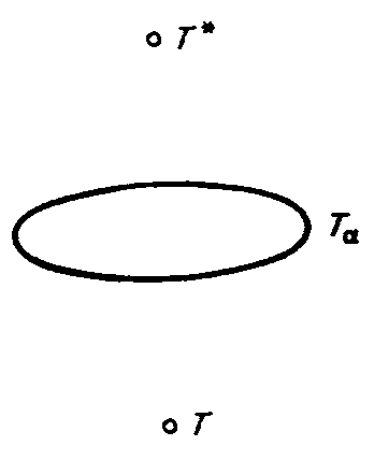
\includegraphics[width = 3 cm]{spectrumTalpha.png}
    \caption{The self-adjoint extensions of $\op T$.}
\end{figure}

\end{example}


%%-------------------------------------
%	BIBLIOGRAPHY
%-------------------------------------

\renewcommand{\refname}{\spacedlowsmallcaps{References}} % For modifying the bibliography heading

\bibliographystyle{unsrt}

\bibliography{sample.bib} % The file containing the bibliography

%------------------------------------

\end{document}
